\chapter{Ergebnis}

In diesem Kapitel wird die konkrete Implementierung meines Test-Frameworks JUUT vorgestellt. Wie man in dem Übersichtsdiagramm auf der nächsten Seite sehen kann, besteht es aus einem Kernel (\textit{Core}) und einem Unity spezifischen Teil auf die ich in den nächsten zwei Sektionen eingehen werde. Zuletzt fasse ich das Erreichte kurz zusammen und vergleiche es mit den existierenden Frameworks.

Im Großen und Ganzen ist die fertige Struktur ähnlich zum \hyperref[fig:WalkingSkeleton]{Erstentwurf} abgesehen davon, dass es einen extra Bereich für die Unity spezifischen Komponenten gibt. Wodurch der Kernel auch für Test-Frameworks andere Spiele-Engines genutzt werden könnte. Das was im Erstentwurf Klassen waren, sind in der fertigen Implementierung meistens eigene Pakete, die die vorgesehene Funktionalität kapseln. Dadurch ist das Projekt offen für Erweiterungen.

\clearpage
\begin{figure}
\centering
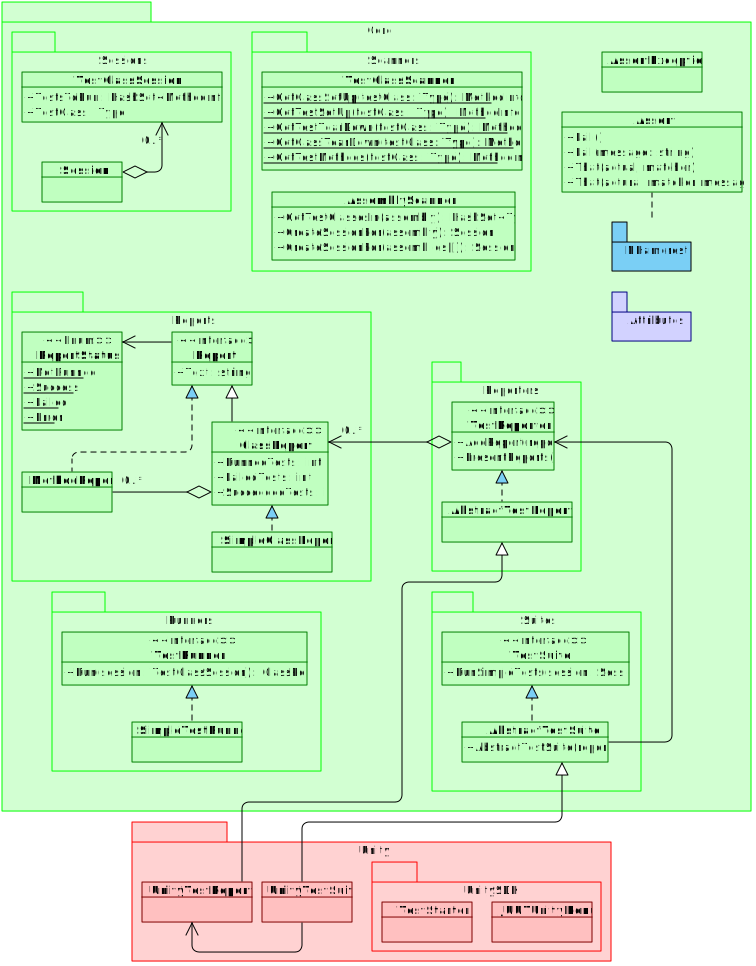
\includegraphics[width=0.9\linewidth]{images/Kapitel_Ergebnis/Overview}
\caption[Übersichtliches Klassendiagramm von JUUT]{Übersichtliches Klassendiagramm von JUUT\\
In diesem Diagramm sind alle Klassen enthalten. Zwecks Übersicht werden nur die wichtigsten Methoden und Attribute dargestellt, sodass man einen Überblick über die Struktur erhält.}
\label{fig:Overview}
\end{figure}
\clearpage

\section{Kernel}

Der Kernel unterteilt sich in mehrere Pakete, welche zu einem bestimmten Aufgabenbereich gehören. Lediglich die Klassen \textit{Assert}, \textit{AssertException} und eine Util-Klasse (welche nicht im Übersichtsdiagramm aufgeführt ist) sind in keinem eigenen Paket.

Die drei Hauptaufgaben des Kernels sind
\begin{itemize}
\item \textbf{Definieren von Tests}\\
Hierfür ist hauptsächlich das Paket \textit{Attributes} zuständig, welches dem Benutzer Attribute zur Verfügung stellt um seine Tests zu markieren. Dazu kommt noch die Klasse \textit{Assert} in Zusammenhang mit der Bibliothek NHamcrest.
\item \textbf{Ausführen der Tests}\\
Die Pakete \textit{Sessions}, \textit{Runners} und \textit{Suites} erfüllen diese Aufgabe, wobei die \textit{Scanner} zu Hilfe genommen werden.
\item \textbf{Präsentation der Testergebnisse}\\
Dies wird von den Paketen \textit{Reports} und \textit{Reporters} durchgeführt. Zusätzlich wird die Klasse \textit{AssertException} verwendet, um den Status eines Testergebnisses zu bestimmen und den Text einer fehlgeschlagenen Bedingung zu formatieren.
\end{itemize}

Wie diese Aufgaben implementiert wurden, möchte ich in den nächsten Abschnitten erläutern.

\subsection{Definieren von Tests}

Zur Definition von Tests stehen dem Benutzer einige Attribute zur Verfügen, mit denen er zum Beispiel Testklassen und Testmethoden markieren kann. Ein ausführliches Klassendiagramm aller Attribute befindet sich auf der nächsten Seite.

Einige der Attributsklassen sind abstrakt und dienen der internen Strukturierung, was für die in späteren Abschnitten erläuterten \textit{Runner} und \textit{Scanner} benötigt wird. Die Wurzel der Hierarchie bildet die abstrakte Klasse \textit{JUUTAttribute} die definiert, dass jedes Attribut einen Namen haben muss, welcher zur Präsentation der Testergebnisse verwendet wird. Außerdem bietet sie eine statische Methode, welche überprüft ob ein beliebiger \textit{Member} (zum Beispiel eine Klasse oder eine Methode) zulässig für das Attribut ist. Deswegen muss jedes nicht-abstrakte Attribut die Methode \textit{Validate} implementieren. Zum Beispiel wird bei einfachen Testmethoden (markiert durch \textit{SimpleTestMethod}) geprüft, dass der Member eine Methode ist und keine Parameter erwartet (s. \autoref{code:SimpleTestMethodAttribute_Validate} \nameref{code:SimpleTestMethodAttribute_Validate}). Hat er allerdings Parameter, wird eine Exception geworfen, um dem Anwender diesen Fehler bei der Präsentation der Testergebnisse mitzuteilen.

\begin{figure}[h]
\centering
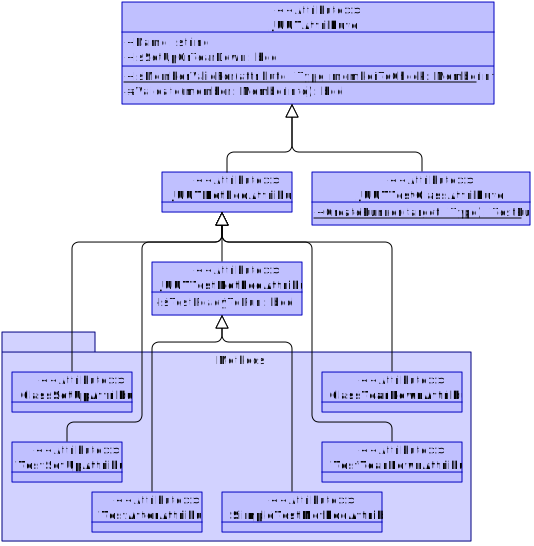
\includegraphics[width=0.9\linewidth]{images/Kapitel_Ergebnis/Attributes}
\caption[Attribute zur Markierung testspezifischer Elemente]{Attribute zur Markierung testspezifischer Elemente}
\label{fig:Attributes}
\end{figure}

Das \textit{JUUTTestClass}-Attribut wir zur Markierung von Testklassen benutzt. Zusätzlich zu den geerbten Funktionalitäten, liefert es auch den optimalen \textit{TestRunner} für die markierter Testklasse. Denn je nachdem welche Arten von Tests diese enthält wird ein anderer Typ \textit{Runner} zur fehlerfreien Ausführung benötigt.

Als abstrakte Superklasse aller Testmethoden dient \textit{JUUTTestMethodAttribute}. Dadurch kann einem der \textit{TestClassScanner} alle Tests einer Testklasse liefern, ohne alle konkreten Test-Attribute zu kennen. Es hat ein öffentlich lesbares Attribut \textit{IsReadyToRun} welches angibt, ob der markiert Test schon ausgeführt werden kann. Dies wird von den \textit{Runnern} berücksichtigt, wodurch komplexere Testmethoden möglich sind. Für konkrete Tests gibt es die Attribute \textit{SimpleTestMethod} und \textit{TestAfter}. Mit Ersterem markiert man einfache Tests, die immer bereit zur Ausführung sind. Diese sind äquivalent zu den Tests die mit UUnit oder SharpUnit möglich sind. Mit \textit{TestAfter} versehene Tests sollen nach der Ausführung einer bestimmten Methode einer Klasse durchgeführt werden (zum Beispiel die \textit{Update}-Methode eines Skripts). Ursprünglich hatte ich vor diese Funktionalität mit Aspektorientierte Programmierung\footnote{Mit AOP lassen sich eigene Funktionalitäten an bestimmte Stellen des Programms einweben. Mehr dazu findet man zum Beispiel in \textit{"`Aspect-oriented programming"} unter anderem von Gregor Kiczales.} zu implementieren. Das Attribut wäre dabei gleichzeitig der \textit{Advice} der nach dem Methodenaufruf eingewoben werden würde und einen \textit{ReadyToRun}-Flag auf wahr setzt, wodurch der \textit{Runner} den Test beim nächsten Durchgang ausführt. Allerdings wird zum Umweben einer nicht statischen Methode einer Klasse ein \textit{Proxy-Objekt} benötigt, welches an Stelle des eigentlichen Objekts verwendet wird. Leider ist es nicht möglich in einer laufenden Unity-Umgebung ein Skript durch ein entsprechendes \textit{Proxy-Objekt} zu ersetzen. Zum Zeitpunkt der Fertigstellung dieser Studienarbeit war es mir nicht möglich dieses Problem zu lösen, sodass diese Funktionalität nur schematisch vorhanden ist.

Neben Attributen für Testmethoden, gibt es noch weitere für \textit{SetUp}- und \textit{TearDown}- Methoden. Von der Definition von Tests entspricht JUUT also dem Funktionsumfang von MSTest.

Abgesehen von den Attributen sind für Tests noch die möglichen Assertions wichtig. Diese werden von der Klasse \textit{Assert} zur Verfügung gestellt.
\begin{wrapfigure}{r}{0.5\linewidth}
\centering
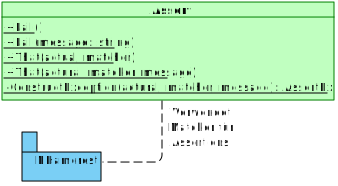
\includegraphics[width=0.95\linewidth]{images/Kapitel_Ergebnis/Assert}
\caption[\textit{Assert}-Klasse von JUUT]{\textit{Assert}-Klasse von JUUT}
\label{fig:Assert}
\end{wrapfigure}
Durch die Verwendung von NHamcrest ist diese sehr schlank und bietet dennoch mehr Bedingungen, auf die getestet werden können, als die Standard-\textit{Assert}-Klassen von UUnit, SharpUnit oder MSTest. So werden nur zwei Methoden benötigt. Zum einen die Methode \textit{Fail}, die den Test gezielt fehlschlagen lässt, indem sie eine \textit{AsserException} wirft. Optional lässt sich diese mit einer Nachricht versehen, welche bei der Präsentation angezeigt wird. Dazu kommt noch die Methode \textit{That}. Diese erwartet das zu überprüfende Objekt \textit{actual} und einen \textit{Matcher}, der überprüft ob dieses eine bestimmte Bedingung erfüllt. Bedingungen können sein, dass \textit{actual} nicht Null ist oder dass von einer Anweisung eine Exception geworfen wird.

Abschließend wird gezeigt, wie ein Test mit JUUT definiert werden kann:
\begin{lstlisting}[caption={[Beispiel für einen Test mit JUUT]Beispiel für einen Test mit JUUT\\In diesem Fall sind \textit{Throws.An} und \textit{Is.NotNull} die Matcher, welche den ersten Parameter darauf überprüfen, dass eine Exception geworfen wird beziehungsweise das Objekt nicht Null ist.}, label=code:SimpleTestMethodAttribute_Validate]
[JUUTTestClass]
public class TestClass {
	
	private ClassToTest objectToTest;
	
	[TestSetUp]
	public void SetUp() {
		objectToTest = new ClassToTest();
	}
	
	[SimpleTestMethod]
	public void TestObjectCreation() {
		Assert.That(() => { new ClassToTest(null); }, Throws.An<ArgumentException>());
		Assert.That(objectToTest.ImportantProperty, Is.NotNull());
	}
		
	[TestSetUp]
	public void SetUp() {
		objectToTest = null;
	}
	
}
\end{lstlisting}
\clearpage

\subsection{Ausführen der Tests}

Das Ausführen der Tests ist die Kernfunktionalität eines Test-Frameworks und wird bei JUUT von den Paketen \textit{Sessions}, \textit{Runners} und \textit{Suites}, unter der Zuhilfenahme der \textit{Scanner}, durchgeführt. Die \textit{Sessions} verwalten die auszuführenden Tests, während \textit{Runner} und die \textit{Suite} für das tatsächliche Testen zuständig sind.

Als erstes muss der Anwender mit \textit{Session}-Objekten definieren, welche Tests durchgeführt werden sollen, weswegen dieses Paket zuerst vorgestellt wird.

\begin{figure}[h]
\centering
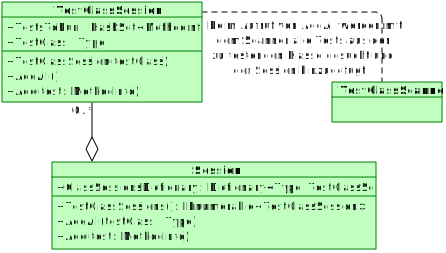
\includegraphics[width=0.8\linewidth]{images/Kapitel_Ergebnis/Sessions}
\caption[\textit{Sessions}-Paket]{\textit{Sessions}-Paket}
\label{fig:Sessions}
\end{figure}

Eine \textit{TestClassSession} repräsentiert eine Testklasse und verwaltet die zu dieser Klasse gehörenden Testmethoden. Sie muss einer mit dem \textit{JUUTTestClass}-Attribut versehenen Klasse zugeordnet werden, weswegen sie als Konstruktor-Parameter einen Typ erwartet. Mit den Methoden \textit{AddAll} und \textit{Add} können alle oder einzelne Testmethoden der Testklasse hinzugefügt werden. Beim Aufruf von \textit{AddAll} durchsucht die statische Hilfsklasse \textit{TestClassScanner} den zugeordneten Typ nach Methoden, welche mit einem \textit{JUUTTestMethod}-Attribut markiert wurden, die dann zur \textit{Session} hinzugefügt werden. Wie das Scannen genau implementiert wurde, sieht man in der Sektion \ref{sec:Appendix_Scanners} \nameref{sec:Appendix_Scanners} im Appendix.

\textit{TestClassSession} dient der JUUT-internen Verwaltung. Vom Anwender muss lediglich eine \textit{Session} erzeugt werden, welche wiederum eine Menge von \textit{TestClassSessions} verwaltet. Diese werden in Form einer Hashtabelle gespeichert, wobei der Schlüssel der Typ der Testklasse und das Element die dazugehörige \textit{TestClassSession} ist. Die Methoden \textit{AddAll} und \textit{Add} von \textit{Session} überprüfen nun, ob es schon eine \textit{TestClassSession} für den hinzuzufügenden Test gibt, erstellen gegebenenfalls eine Instanz und delegieren dann an das \textit{TestClassSession}-Objekt. Die Definition einer \textit{Session} könnte wie folgt aussehen:
\begin{lstlisting}[caption={[Beispiel für die Definition einer \textit{Session}]Beispiel für die Definition einer \textit{Session}}, label=code:Example_SessionCreation]
Session session = new Session();
session.AddAll(typeof(TestClass));
session.Add(typeof(AnotherTestClass).GetMethod("ATestMethod"));
\end{lstlisting}

Nachdem eine \textit{Session} definiert wurde, müssen die darin enthaltenen Tests ausgeführt werden. Diese Aufgabe übernimmt die \textit{TestSuite} und weitere Klassen, welche im nachfolgenden Klassendiagramm dargestellt sind.

\begin{figure}[h]
\centering
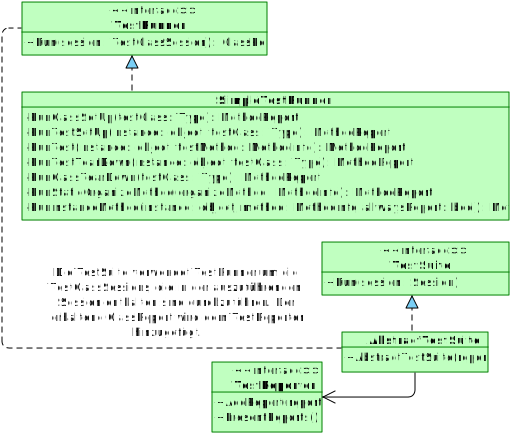
\includegraphics[width=0.8\linewidth]{images/Kapitel_Ergebnis/SuitesAndRunners}
\caption[Für die Ausführung von Tests verantwortliche Klassen]{Für die Ausführung von Tests verantwortliche Klassen}
\label{fig:SuitesAndRunners}
\end{figure}

Eigentlich führen die \textit{TestRunner} die Tests durch, da die \textit{TestSuite} für jede in der \textit{Session} enthaltene \textit{TestClassSession} an einen \textit{TestRunner} delegiert. Der zurückgegebene \textit{ClassReport} wird dem \textit{TestReporter} hinzugefügt und nach Abschluss wird dessen \textit{PresentReports}-Methode aufgerufen um die Ergebnisse darzustellen. Der Ablauf innerhalb des \textit{TestRunners} ist wie folgt:
\begin{enumerate}
\item Erzeugung einer \textit{ClassReport}-Instanz
\item Aufruf der \textit{ClassSetUp}-Methode
\item Erzeugung einer Instanz der zu testenden Klasse
\item Für jeden Test der \textit{TestClassSession}
	\begin{enumerate}[label*=\arabic*.]
	\item Aufruf der \textit{TestSetUp}-Methode
	\item Aufruf der Testmethode
	\item Aufruf der \textit{TestTearDown}-Methode
	\end{enumerate}
\item Aufruf der \textit{ClassTearDown}-Methode
\item Rückgabe des gefüllten \textit{ClassReports}
\end{enumerate}

Die einzelnen Methodenaufrufe werden mit Hilfe von \textit{Reflection} durchgeführt. Falls dabei eine Exception geworfen wird, wird diese gefangen und daraus ein \textit{MethodReport} erzeugt, welcher der \textit{ClassReport}-Instanz hinzugefügt wird. Tritt ein Fehler in einer der organisierenden Methoden (z.B. \textit{TestSetUp} oder \textit{TestTearDown}) auf, wird der Durchlauf abgebrochen und der Bericht sofort zurückgegeben, da der Fehler bei jeder einzelnen Testmethode auftreten würde. Die konkrete Implementierung findet man in der Sektion \ref{sec:Appendix_Runners} \nameref{sec:Appendix_Runners} im Appendix.

Eine \textit{Session} lässt sich nun mit folgendem Code ausführen:
\begin{lstlisting}[caption={[Beispiel für die Ausführung einer \textit{Session}]Beispiel für die Ausführung einer \textit{Session}\\\textit{ConcreteTestSuite} ist stellvertretend für eine beliebige Implementierung von \textit{AbstractTestSuite}.}, label=code:Example_SessionCreation]
Session session = new Session();
session.AddAll(typeof(TestClass));
session.Add(typeof(AnotherTestClass).GetMethod("ATestMethod"));

TestSuite suite = new ConcreteTestSuite();
suite.Run(session);
\end{lstlisting}
\clearpage

\subsection{Präsentation der Testergebnisse}

Nachdem die Tests durchgeführt wurden, müssen die Ergebnisse nur noch dem Benutzer präsentiert werden. Da die Form der Präsentation abhängig von der Spiele-Engine ist, worauf in \autoref{sec:Ergebnis_Unity} näher eingegangen wird, beschäftigt sich dieser Teil mit der Strukturierung und Verwaltung der einzelnen Berichte.

\section{Unity}
\label{sec:Ergebnis_Unity}

\section{Zusammenfassung}